\section{$\phi$-meson analysis} 
\subsection{Basic information}

The dataset used for this $\phi$-meson analysis is taken from year 2018, the single beam energy is about 3.85 GeV with translated to $\sqrt{s_{NN}}$ = 3.0 GeV. The total number of statistics is about $\sim$260M events after event cut selection. The trigger used here is bbce\_tof main trigger with id equal to 620052. Basically, the event level information is same as the $\pi,K,p$ analysis.

\subsection{Particle reconstruction}

$\phi$-mesons are reconstructed through the typically hadronic channel $K^{+}K^{-}$. In the following we will describe the daughter selection and show the $\phi$-meson signals for different $p_T$ and centrality bins. We will also discuss the combining backgrounds estimated with the mixed event technique and like-sign method.

$\phi$-meson decaying to $K^{+}K^{-}$ is strong decay, which it has a relative short lifetime. Thus the primary tracks for daughter selection are used in this analysis. The transverse momentum are required to $\geq$ 0.2 GeV/$c$ to ensure that the track can pass through the TPC, the number of hit points (nHits) along the track is $\geq$ 20 (of a maximum of 45) to ensure good momentum resolution.

The kaon tracks are identified by combining Time Projection Chamber (TPC) and Time Of Flight detector (TOF). The TPC provides particle identification utilizing the energy loss information $dE/dx$. In additional, different particle species with the same momentum have different velocities, thus the TOF can be used to identify different particle species in the $dE/dx$ crossover regions by precise velocity information ($1/\beta$ = $ct/l$). The normalized $dE/dx$, $n\sigma_K$, defined in Eq.~\ref{nsigma}, instead of $dE/dx$ is used in this analysis. Where $\langle{dE/dx}\rangle_{measured}$ and $\langle{dE/dx}\rangle_{K}$ represent measured and theoretical $dE/dx$, and $R$ is the STAR TPC $dE/dx$ resolution (typically $\sim$8\%). The $n\sigma_K$ should be close to a standard Gaussian distribution for each corresponding particle species (mean $=$ 0, $\sigma = $ 1).
\begin{equation}
  n\sigma_x = \frac{1}{R}log\frac{\langle{dE/dx}\rangle_{measured}}{\langle{dE/dx}\rangle_{x}}
\label{nsigma}
\end{equation}

Fig.~\ref{fig:tpcPID} shows the TPC energy loss dE/dx information versus momentum achieved from Run18 Au+Au 3GeV, there are several clear bands for different particle species such as $\pi$, K, p and e. 

Fig.~\ref{fig:tofPID} shows the TOF $m^2$ information versus momentum achieved from Run18 Au+Au 3GeV, also there are several clear bands for different particle species such as $\pi$, K, p . 

\begin{figure}[htbp]
\centering
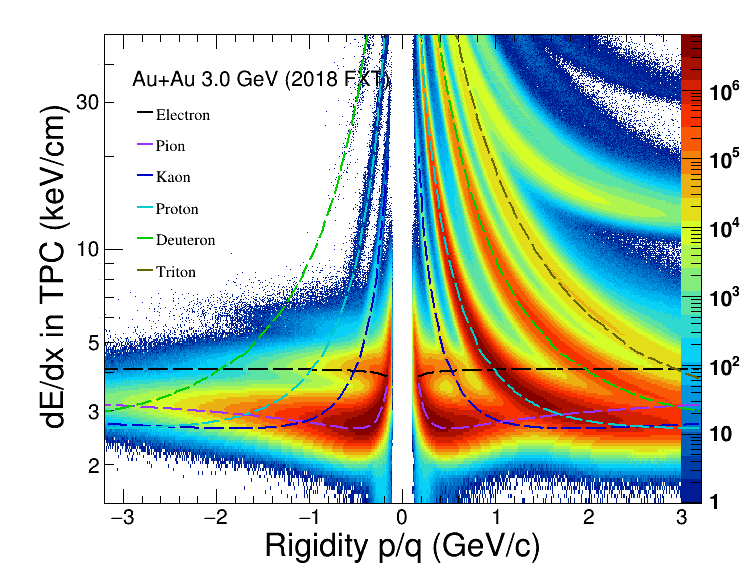
\includegraphics[keepaspectratio,width=0.8\textwidth]{chapterY/fig/3gevDedx.png}
\caption{TPC dE/dx versus charge$\times$momentum achieved from Run18 Au+Au 3GeV.}
 \label{fig:tpcPID}
\end{figure}

\begin{figure}[htbp]
\centering
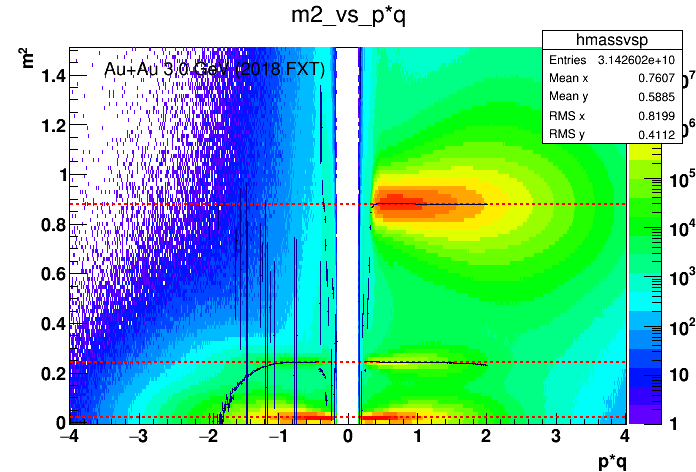
\includegraphics[keepaspectratio,width=0.8\textwidth]{chapterY/fig/3gev_m2_p.png}
\caption{TOF 1/Beta versus momentum achieved from Run18 Au+Au 3GeV.}
 \label{fig:tofPID}
\end{figure}

In summary, next list all the related track selections for $\phi$-meson daughters including track quality cut and particle identification cut.
\begin{itemize}
\item primary tracks
\item $p_{T}$ > 0.2 GeV/$c$
\item $|\eta| < 2$
\item $|Dca| < 3$
\item $nHitsFit \ge 20$, in TPC
\item $nHitsRatio \ge 0.52$, in TPC
\end{itemize}

kaon PID:
\begin{itemize}
  \item $|n\sigma_{K}| < 2.5 $, based on TPC dE/dx
  \item for $K^{+}$, If TOF is avaliable (hybrid PID):  $|\frac{1}{\beta}-\frac{1}{\beta_{exp}}|<0.03$
  \item for $K^{-}$, always require TOF (strict PID):  $|\frac{1}{\beta}-\frac{1}{\beta_{exp}}|<0.03$
\end{itemize}


For the raw yield extraction, the central value was from the fitting method. After the normalized mixed Event background subtraction, we use a breit-wigner + pol1 function to extract the raw signal yield. The statistics error was propagate from the fitting. 

Fig.~\ref{fig:mixedEvent_pT0} to Fig.~\ref{fig:mixedEvent_pT9} show the invariant mass distribution for the foreground and two different uncorrelated backgrounds: same event like-sign and mixed event unlike-sign in different $p_T$ bins include low $p_T$ to high $p_T$. The mixed event backgrounds have been scaled to the foreground using the integration range $m_{K\pi}\in[1.04,1.08]$ GeV/$c^{2}$. Fig.~\ref{fig:mixedEvent_mean} and Fig.~\ref{fig:mixedEvent_width} show the signal mean value and width distribution along $p_T$. 

\begin{figure}[htbp]
\begin{minipage}[htbp]{0.55\linewidth}
\centering
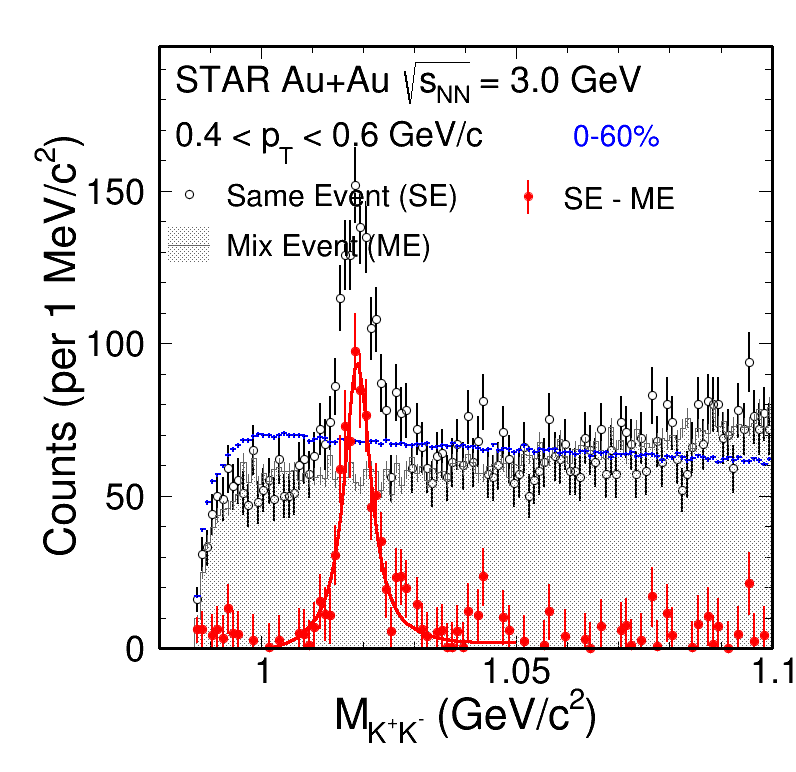
\includegraphics[width=0.95\textwidth]{chapterY/fig/fig1_signal_0_0.png}
\caption{Inv. mass dist. in 0.4 < $p_T$ < 0.6 GeV/$c$. \label{fig:mixedEvent_pT0}}
\end{minipage}
\hfill
\begin{minipage}[htbp]{0.55\linewidth}
\centering
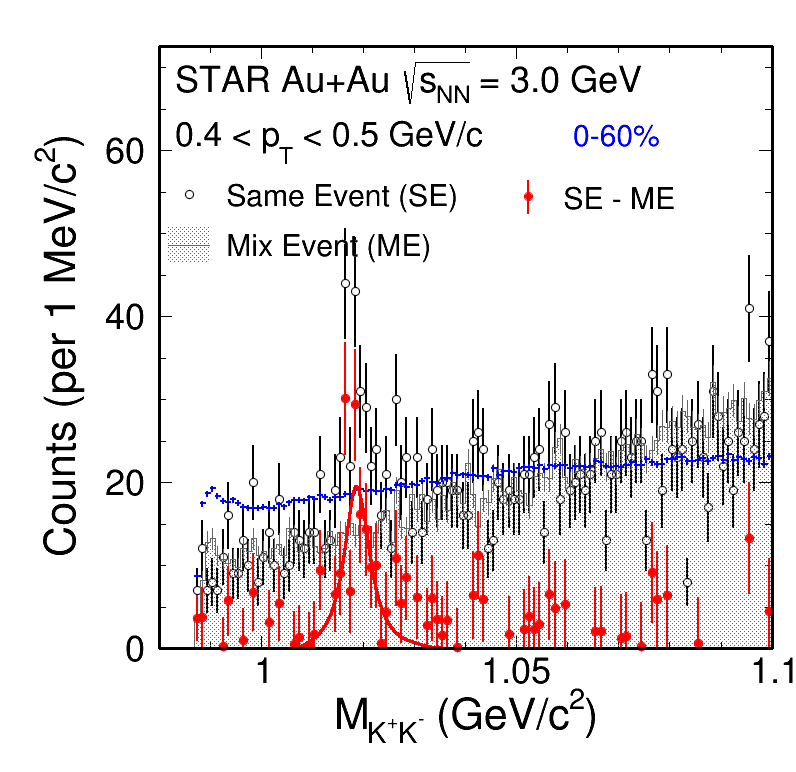
\includegraphics[width=0.95\textwidth]{chapterY/fig/fig1_signal_0_1.png} 
\caption{Inv. mass dist. in 0.4 < $p_T$ < 0.5 GeV/$c$. \label{fig:mixedEvent_pT1}}
\end{minipage}
\end{figure}

\begin{figure}[htbp]
\begin{minipage}[htbp]{0.55\linewidth}
\centering
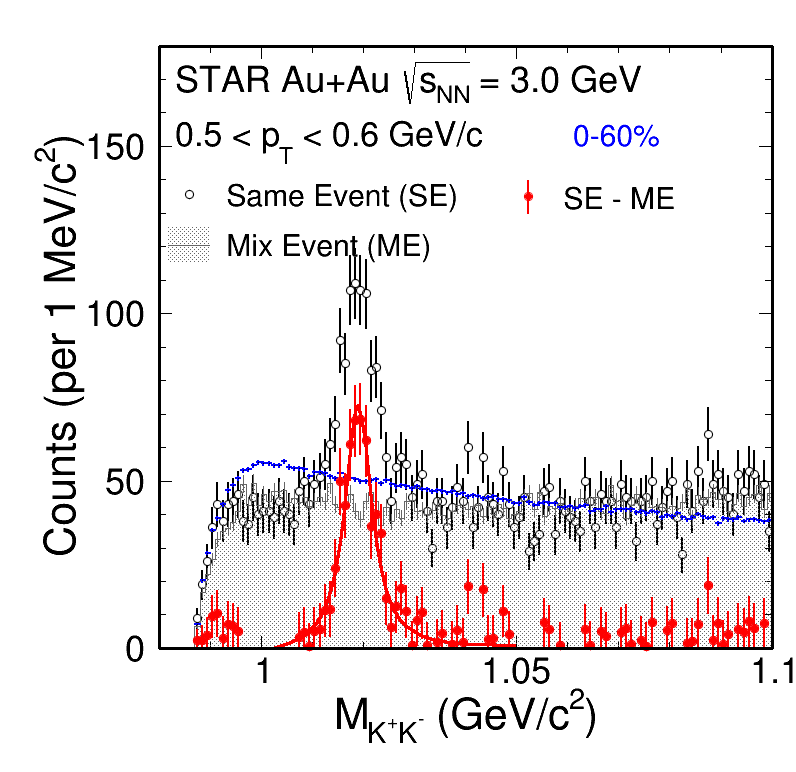
\includegraphics[width=0.95\textwidth]{chapterY/fig/fig1_signal_0_2.png}
\caption{Inv. mass dist. in 0.5 < $p_T$ < 0.6 GeV/$c$. \label{fig:mixedEvent_pT2}}
\end{minipage}
\hfill
\begin{minipage}[htbp]{0.55\linewidth}
\centering
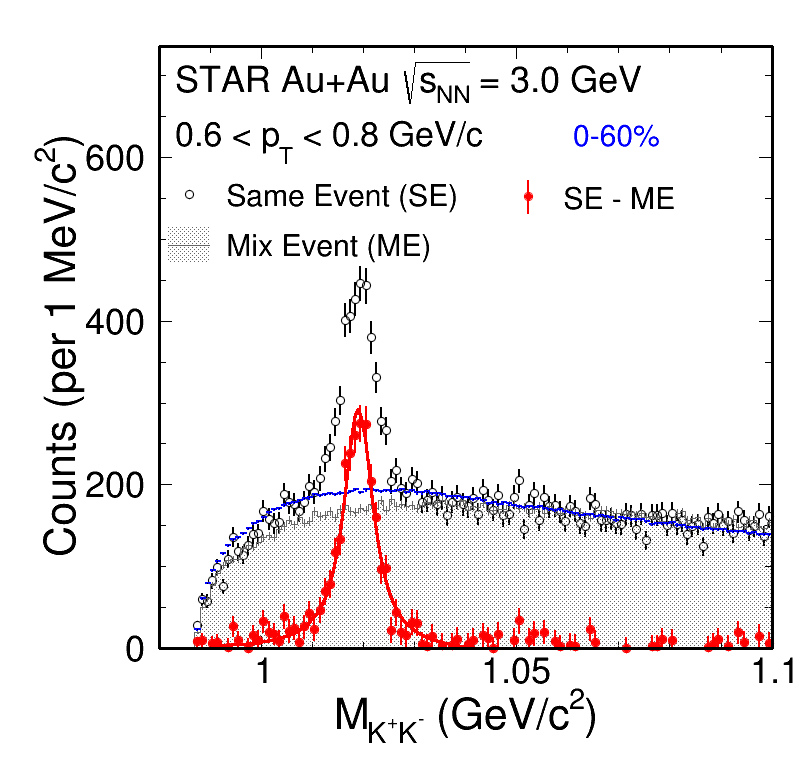
\includegraphics[width=0.95\textwidth]{chapterY/fig/fig1_signal_0_3.png} 
\caption{Inv. mass dist. in 0.6 < $p_T$ < 0.8 GeV/$c$. \label{fig:mixedEvent_pT3}}
\end{minipage}
\end{figure}

\begin{figure}[htbp]
\begin{minipage}[htbp]{0.55\linewidth}
\centering
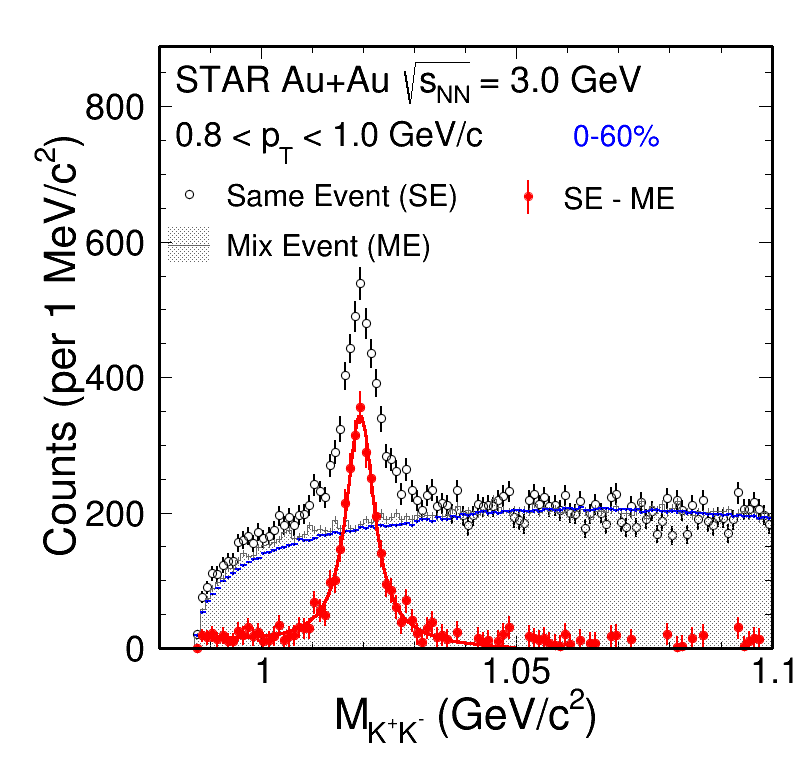
\includegraphics[width=0.95\textwidth]{chapterY/fig/fig1_signal_0_4.png}
\caption{Inv. mass dist. in 0.8 < $p_T$ < 1.0 GeV/$c$. \label{fig:mixedEvent_pT4}}
\end{minipage}
\hfill
\begin{minipage}[htbp]{0.55\linewidth}
\centering
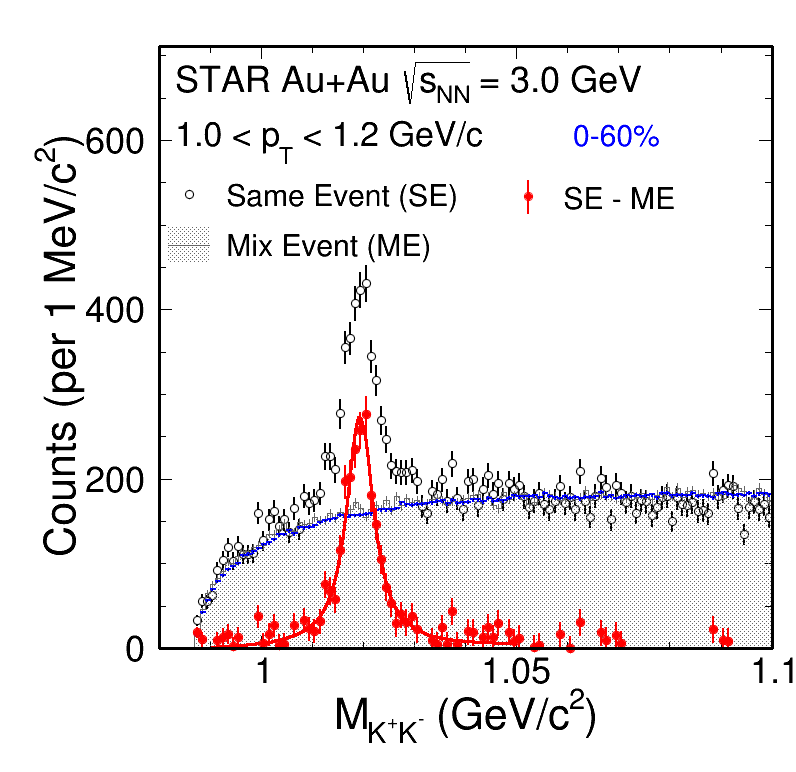
\includegraphics[width=0.95\textwidth]{chapterY/fig/fig1_signal_0_5.png} 
\caption{Inv. mass dist. in 1.0 < $p_T$ < 1.2 GeV/$c$. \label{fig:mixedEvent_pT5}}
\end{minipage}
\end{figure}

\begin{figure}[htbp]
\begin{minipage}[htbp]{0.55\linewidth}
\centering
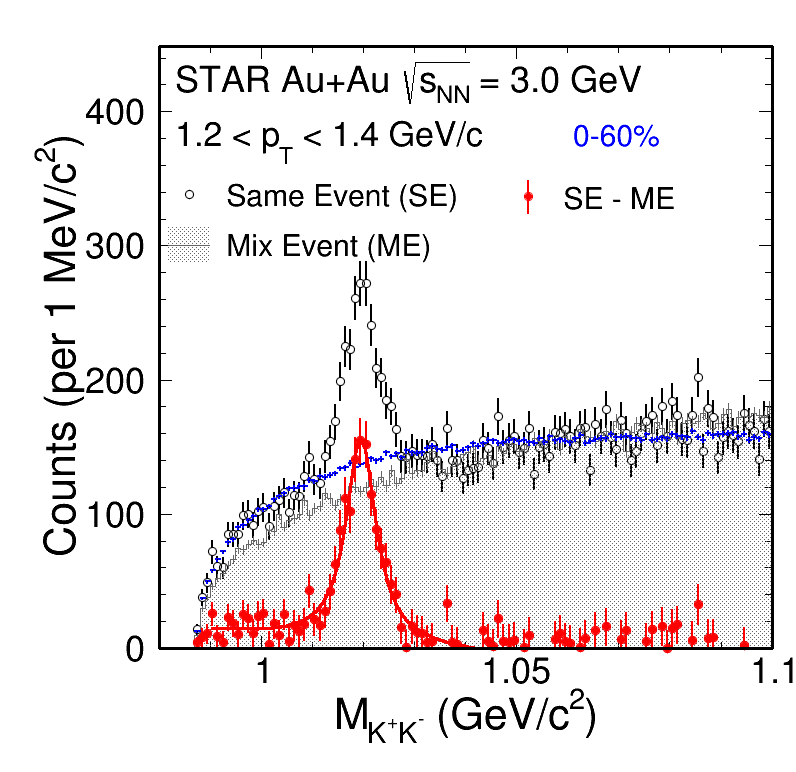
\includegraphics[width=0.95\textwidth]{chapterY/fig/fig1_signal_0_6.png}
\caption{Inv. mass dist. in 1.2 < $p_T$ < 1.4 GeV/$c$. \label{fig:mixedEvent_pT6}}
\end{minipage}
\hfill
\begin{minipage}[htbp]{0.55\linewidth}
\centering
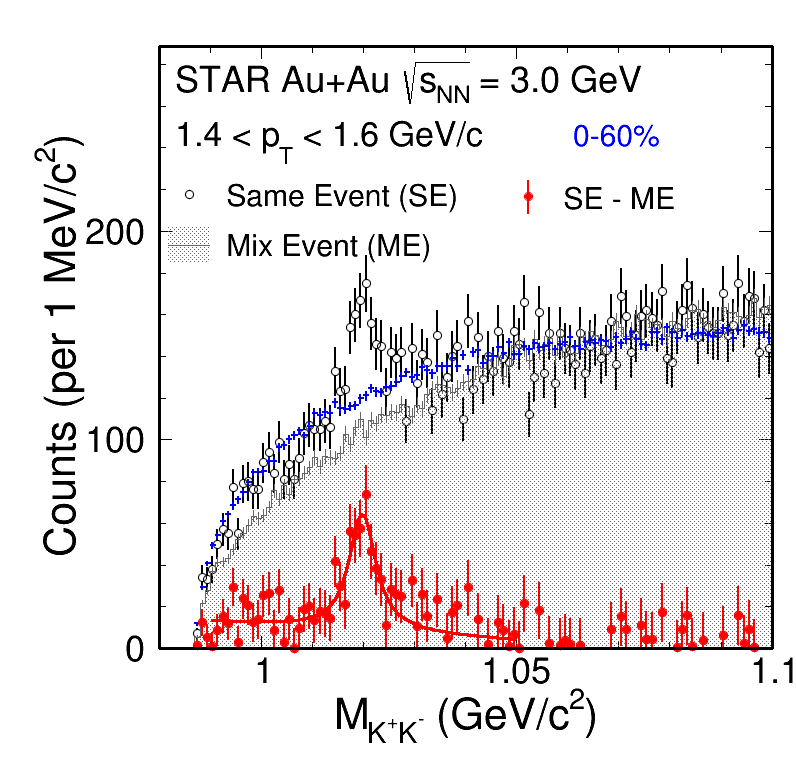
\includegraphics[width=0.95\textwidth]{chapterY/fig/fig1_signal_0_7.png} 
\caption{Inv. mass dist. in 1.4 < $p_T$ < 1.6 GeV/$c$. \label{fig:mixedEvent_pT7}}
\end{minipage}
\end{figure}

\begin{figure}[htbp]
\begin{minipage}[htbp]{0.55\linewidth}
\centering
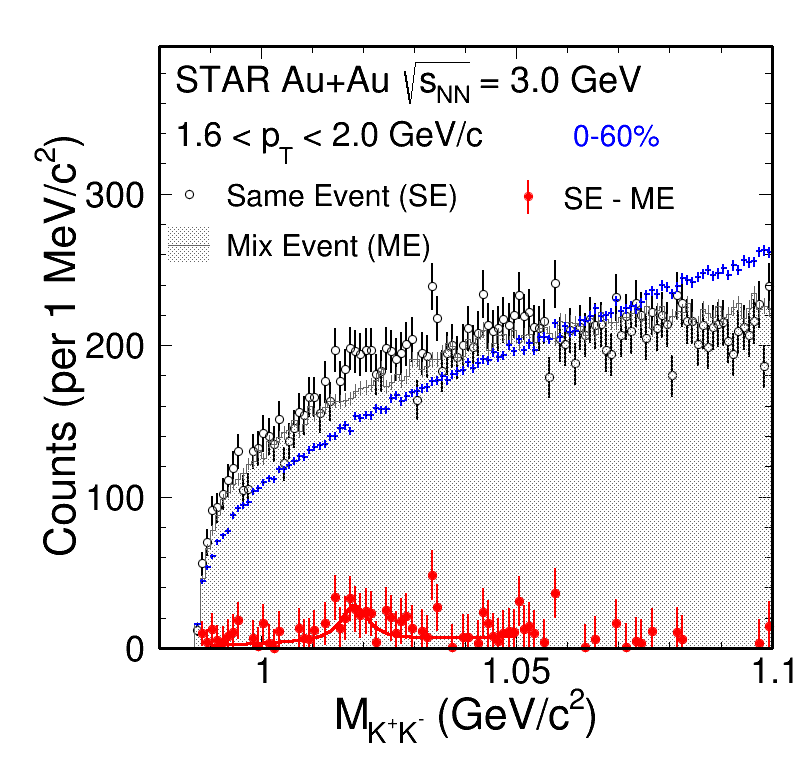
\includegraphics[width=0.95\textwidth]{chapterY/fig/fig1_signal_0_8.png}
\caption{Inv. mass dist. in 1.6 < $p_T$ < 2.0 GeV/$c$. \label{fig:mixedEvent_pT8}}
\end{minipage}
\hfill
\begin{minipage}[htbp]{0.55\linewidth}
\centering
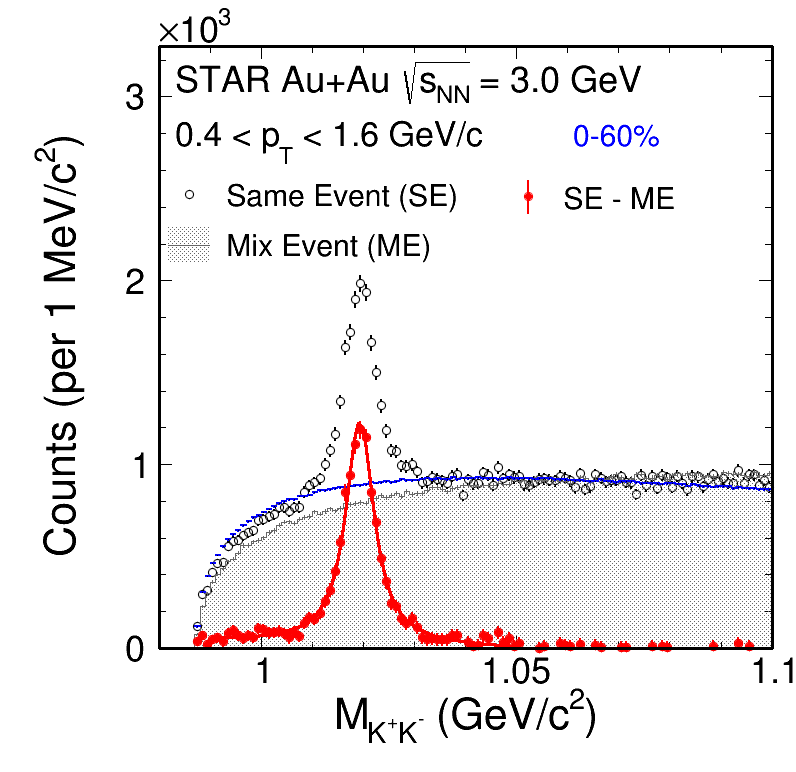
\includegraphics[width=0.95\textwidth]{chapterY/fig/fig1_signal_0_9.png} 
\caption{Inv. mass dist. in 0.4 < $p_T$ < 1.6 GeV/$c$. \label{fig:mixedEvent_pT9}}
\end{minipage}
\end{figure}

\begin{figure}[htbp]
\begin{minipage}[htbp]{0.55\linewidth}
\centering
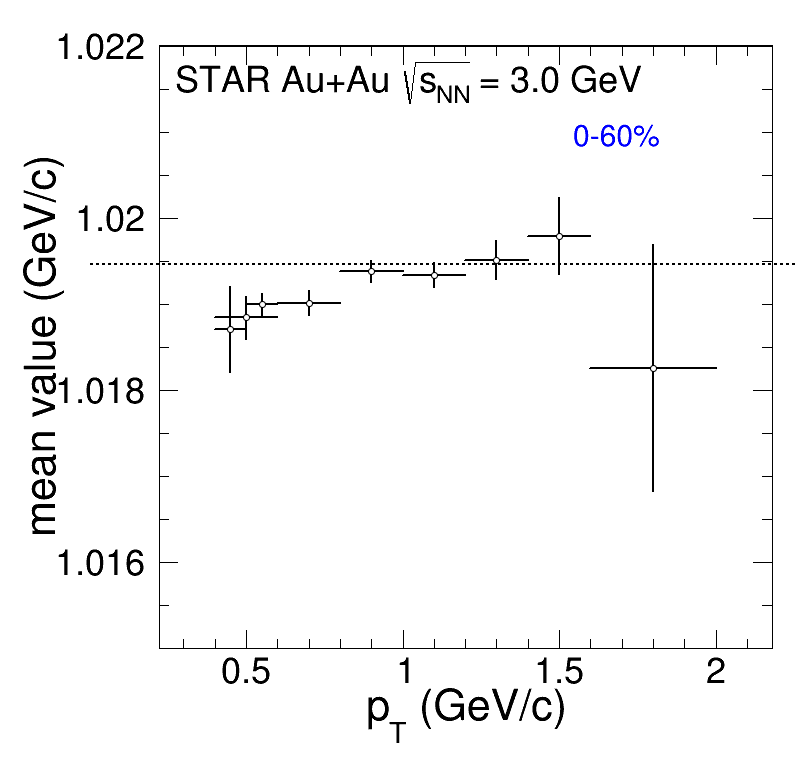
\includegraphics[width=0.95\textwidth]{chapterY/fig/fig1_mean_0.png}
\caption{$\phi$-meson signals mean value along with $p_T$. \label{fig:mixedEvent_mean}}
\end{minipage}
\hfill
\begin{minipage}[htbp]{0.55\linewidth}
\centering
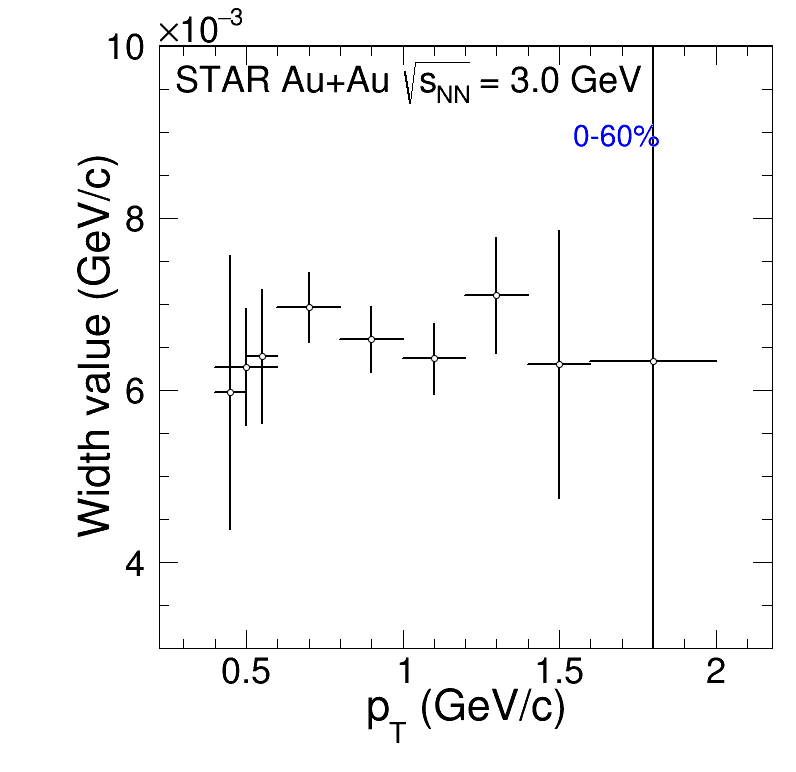
\includegraphics[width=0.95\textwidth]{chapterY/fig/fig1_width_0.png} 
\caption{$\phi$-meson signals width value along with $p_T$. \label{fig:mixedEvent_width}}
\end{minipage}
\end{figure}

For the backgrounds estimation, we have tried two methods, mixed event technique and like-sign pair technique. To construct the mixed event background it is important to combine events with some degree of similarity, such as events are classified according to the centrality class. Nine centrality classes between 0-80\%, are classified for mixing. For the same-event like-sign background method, we also tried, but as clearly the background fluctuation was large compared to the mix-event method. And also due to the asymmetric charge in the low energy collisions. At some certain ranges, these like-sign method can't well describe the background. Thus why the mixed event method is chosen.

Basically, the techical is same as the $\phi$-meson spectra analysis. 

\subsection{Acceptance and efficiency}
\subsubsection{Acceptance}

\begin{figure}[h]
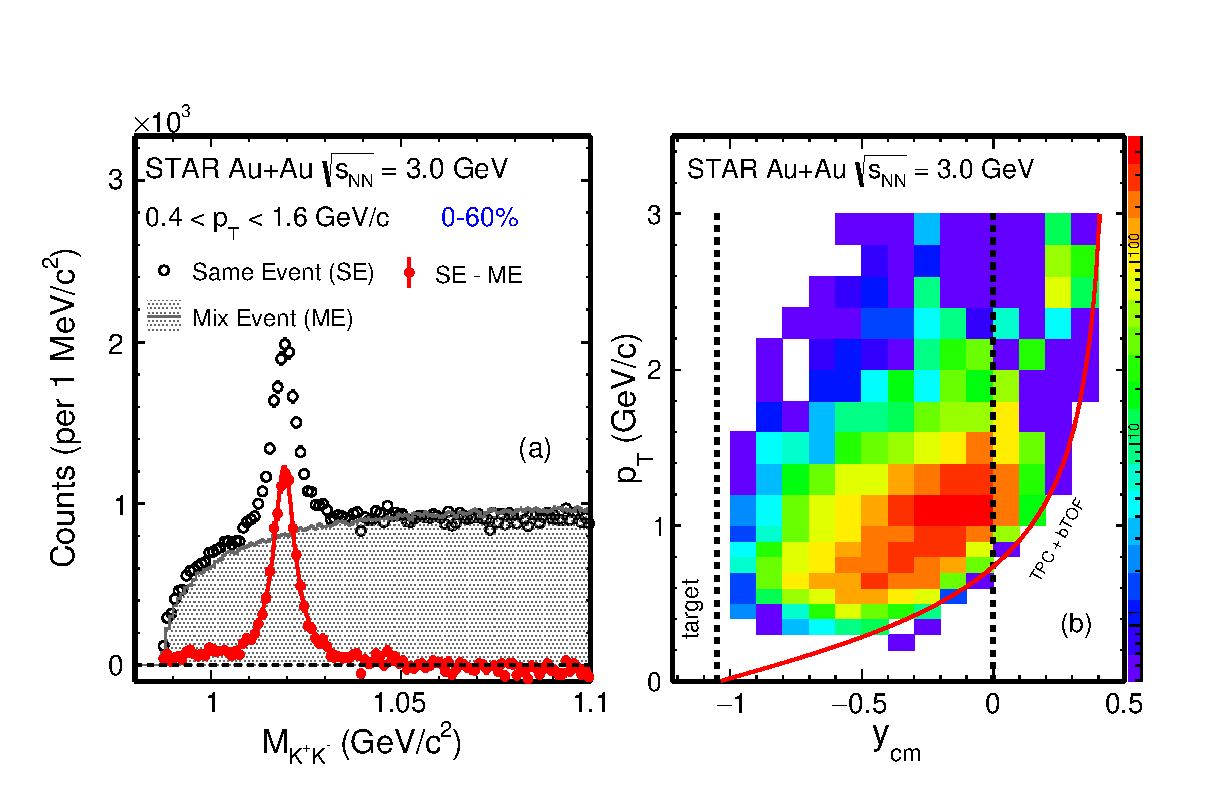
\includegraphics[width=0.85\linewidth]{chapterY/fig/fig1_signal.eps}
  \caption{(a) Invariant mass of $K^+K^-$ pairs in 0-60\% centrality and 0.4--1.6\,GeV/$c$ for the total inclusive yield. (b) The reconstructed $\phi$-meson acceptance $p_T$ vs. rapidity in the center-of-mass frame ($y_{\rm cm}$).}
\label{phiSignal}
\end{figure}

Fig.~\ref{phiSignal} shows the invariant mass of $K^+K^-$ pairs for total inclusive one. Black open circles represent the same-event (SE) unlike-sign (US) distributions. Grey shaded histograms represent the mix-event (ME) US distributions that are used to estimate the combinatorial background. The red solid circles depict the $\phi$-meson signals obtained by subtracting the ME combinatorial background from the SE distributions. (b) The reconstructed $\phi$-meson acceptance $p_T$ vs. rapidity in the center-of-mass frame ($y_{\rm cm}$).


\subsubsection{Efficiency corrections}

\begin{figure}[h]
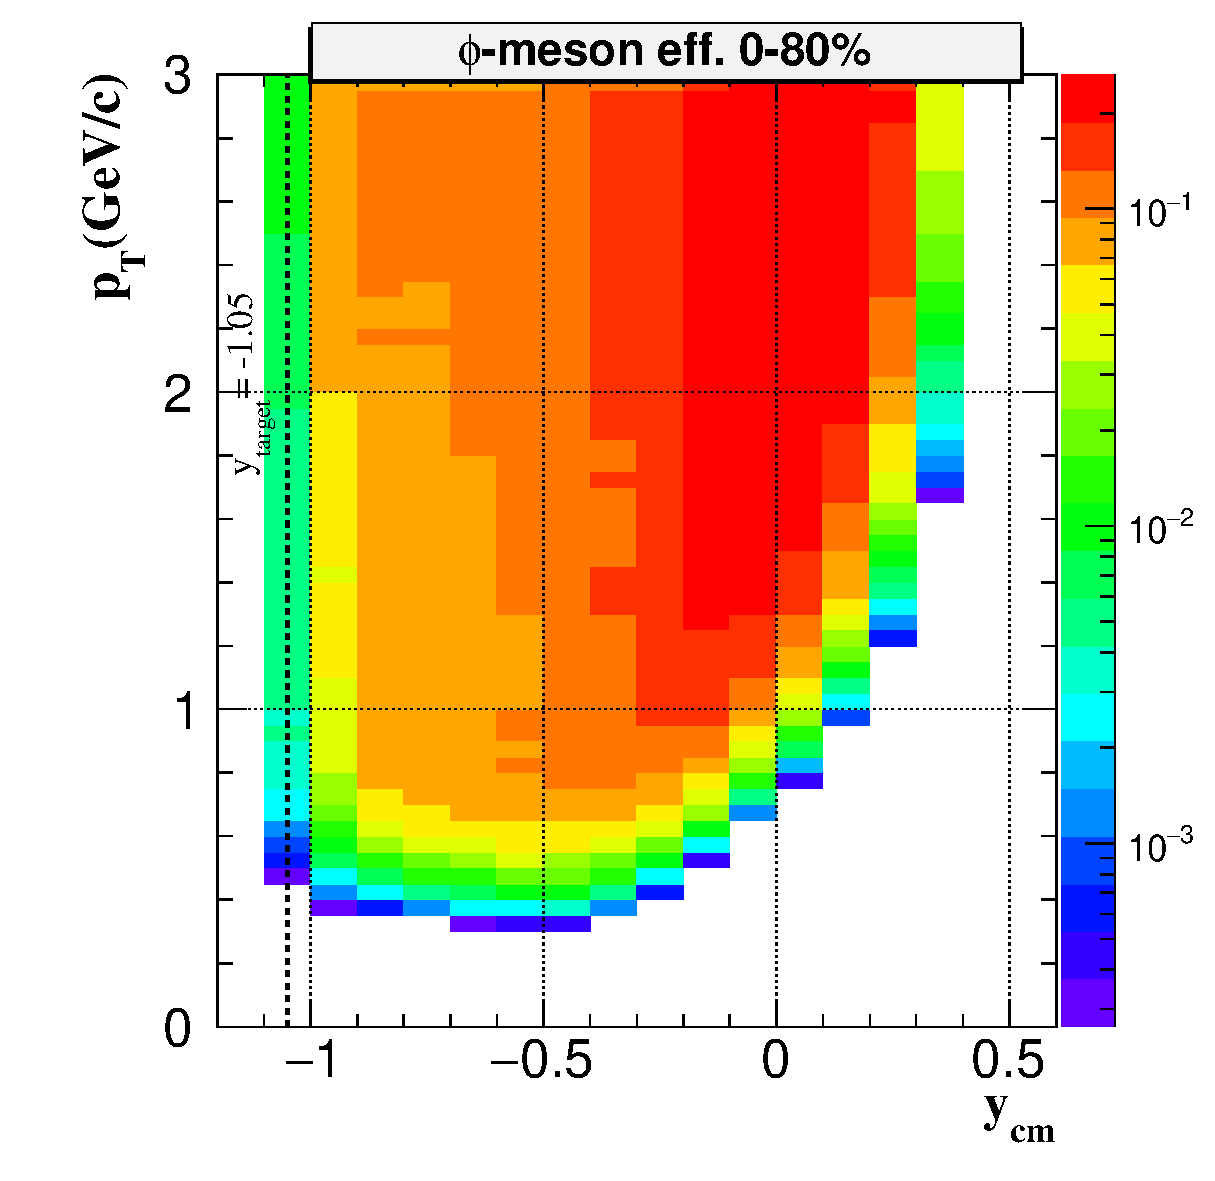
\includegraphics[width=0.6\linewidth]{chapterY/fig/2effAll_rap_0.eps}
\caption{Reconstruction efficiency of $\phi$, as a function of $y$ and $p_{\rm{T}}$ at $\sqrt{s_{NN}}$ = 3 GeV.}
\label{phi_2Deff}
\end{figure}

Fig.~\ref{phi_2Deff} shows the 2D y vs $p_T$ $\phi$-meson reconstruction efficiency used as a re-weight factor for the flow analysis to consider the acceptance effect.


\subsection{$v_1$ and $v_2$ extraction and systematic uncertainties}

\subsubsection{$v_1$}

$\phi$-meson was divided into 6 $\phi$-$\Psi_{1}$ range as shown in Fig.~\ref{phi_v1} from [0, $\pi$], for each range, after the combinatorial background subtracting, a breit-wigner function was used for fitting to extract the raw counts in each individual range. After that, the raw counts was fitted with the function \ref{equ:equation_v1} to extract the raw $v_1$ as shown in Fig.~\ref{phi_v1_fit}. After correct the event plan resolution, the corrected $v_1$ was obtained.

\begin{equation}
  \frac{dN}{d\phi-\Psi_1} \propto 1+2v_1 cos(\phi-\Psi_{1}),
\label{equ:equation_v1}
\end{equation}


\begin{figure}[h]
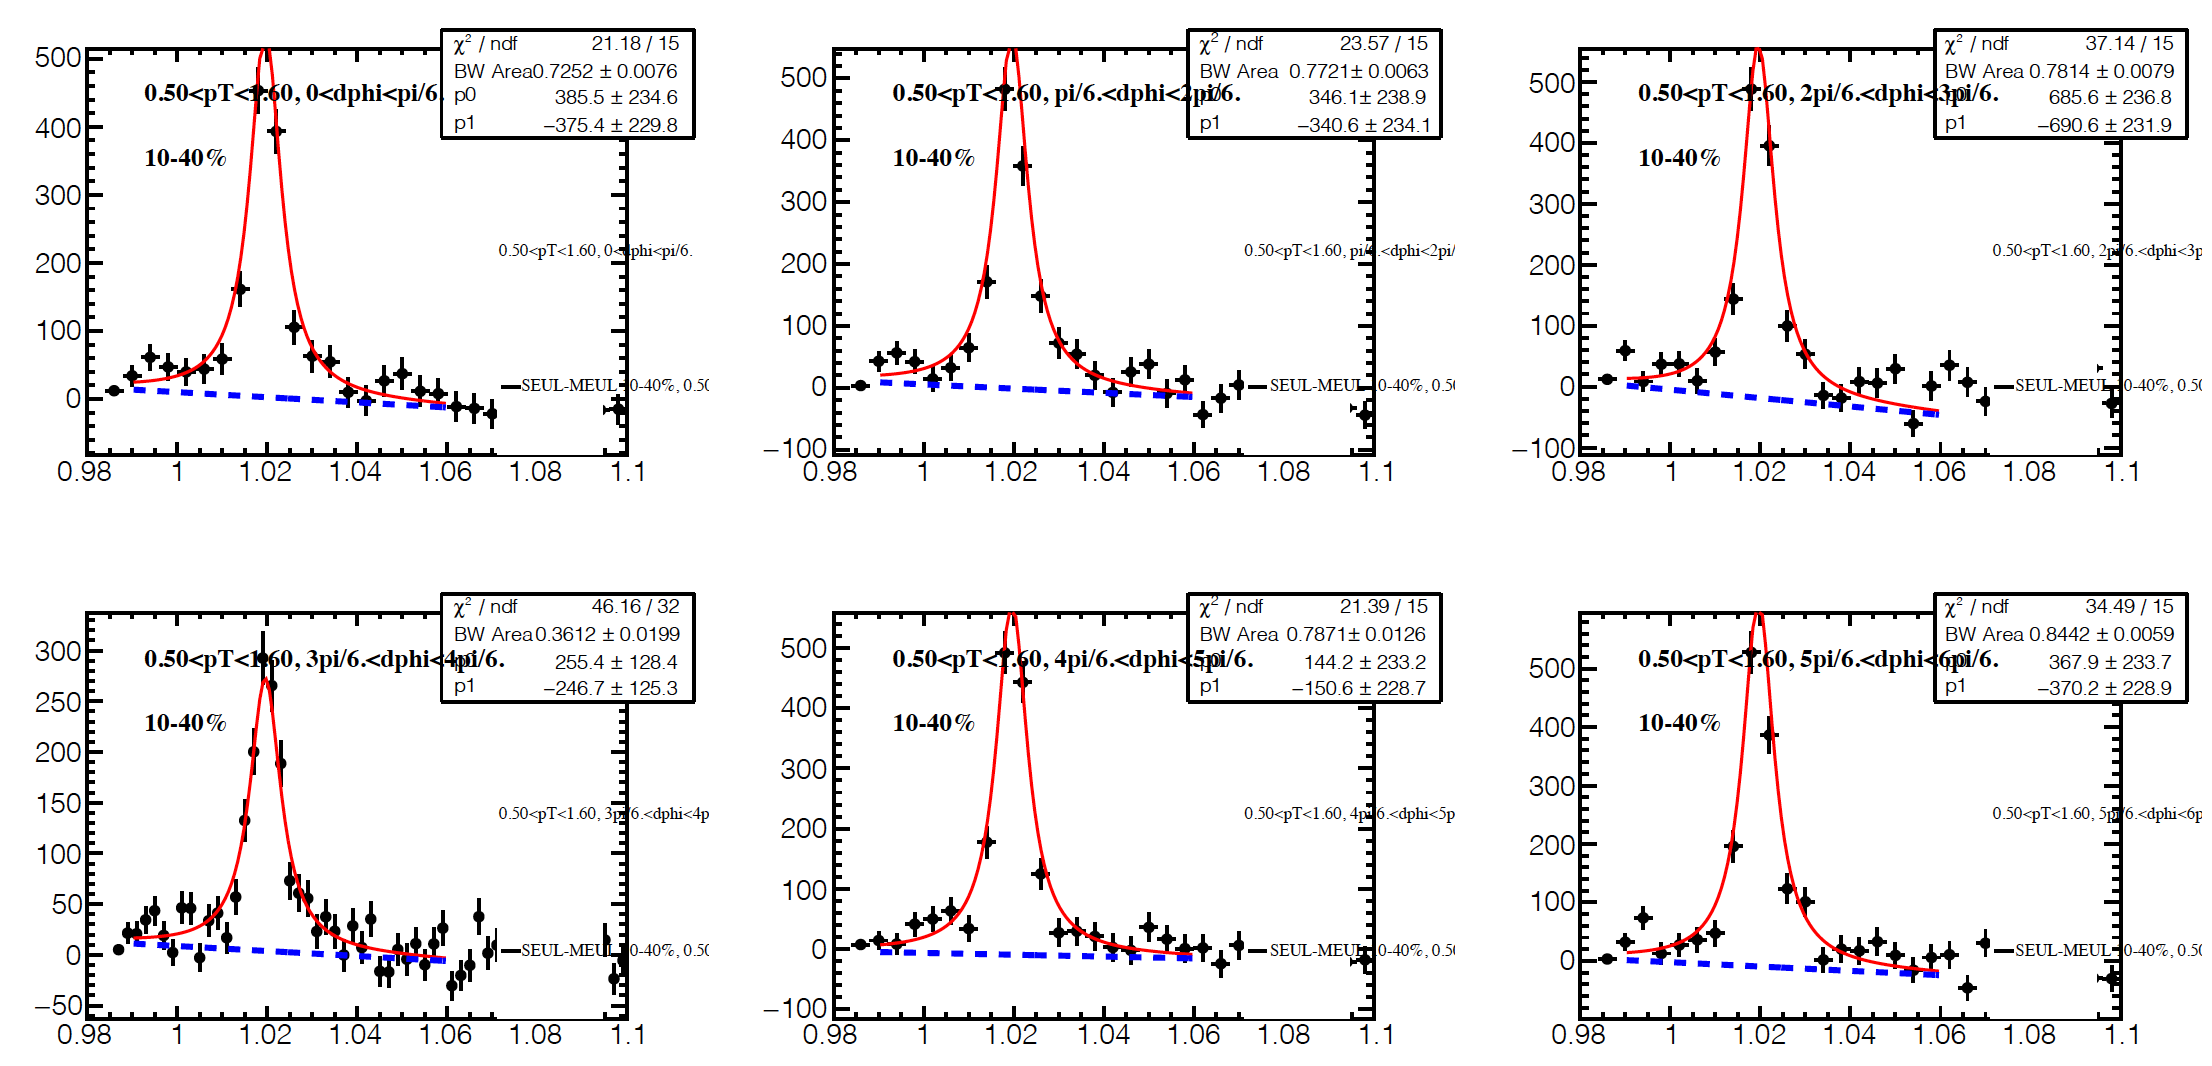
\includegraphics[width=0.98\linewidth]{chapterY/fig/phi_invEP_v1_10_40.png}
\caption{$\phi$-meson signals in several different $\phi$-$\Psi$ range used for the $v_1$ extraction.}
\label{phi_v1}
\end{figure}

\begin{figure}[h]
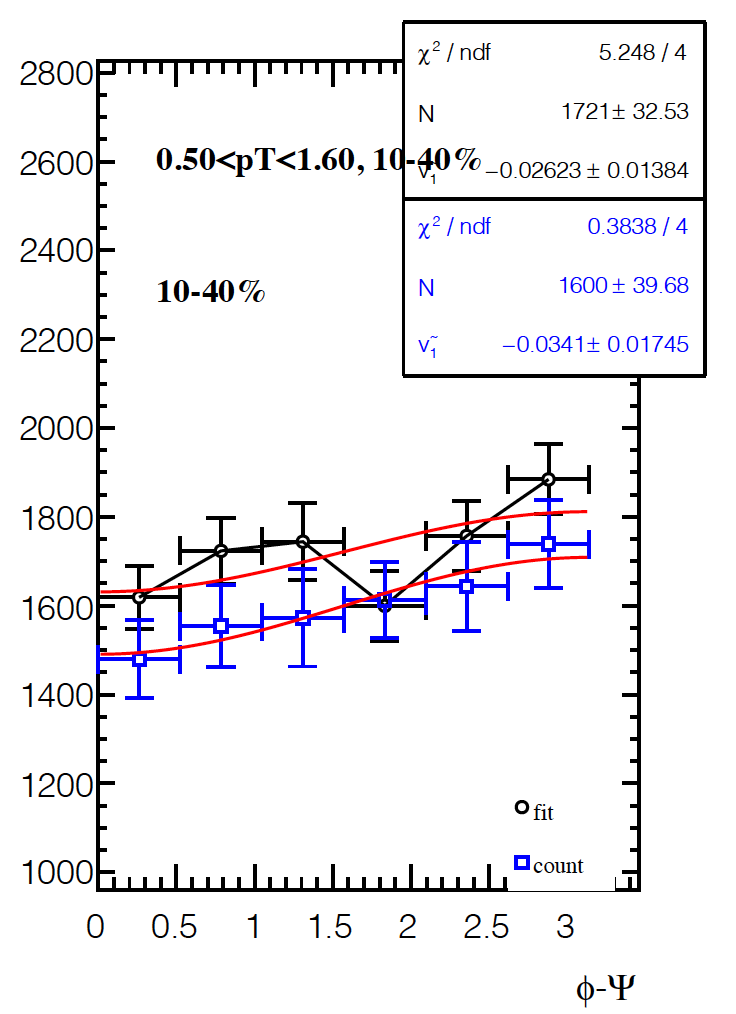
\includegraphics[width=0.55\linewidth]{chapterY/fig/phi_invEP_v1_10_40_fit.png}
  \caption{$\phi$-meson raw counts vs. $\phi$-$\Psi$, fitted with the function to extract the raw v1.}
\label{phi_v1_fit}
\end{figure}

Fig.~\ref{phi_dv1dy} shows an example of the extracted $\phi$-meson $v_1$ along with the rapidity dependence. A linear function which cross (0,0) was used to fitting and obtain the $dv_{1}$/$dy$ slop.

\begin{figure}[h]
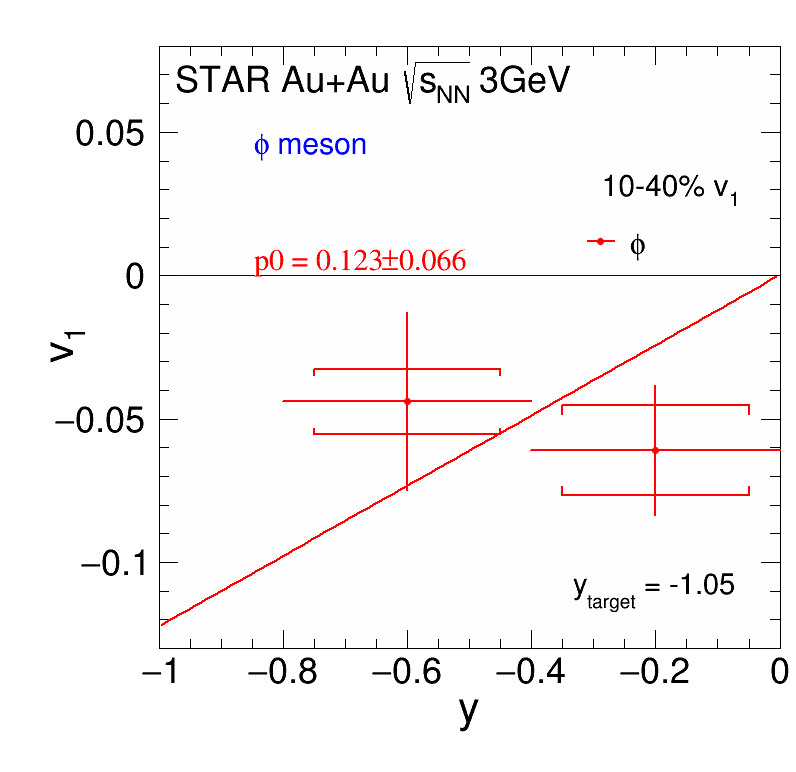
\includegraphics[width=0.49\linewidth]{chapterY/fig/fig1_phi_v1Slop1_10_40.png}
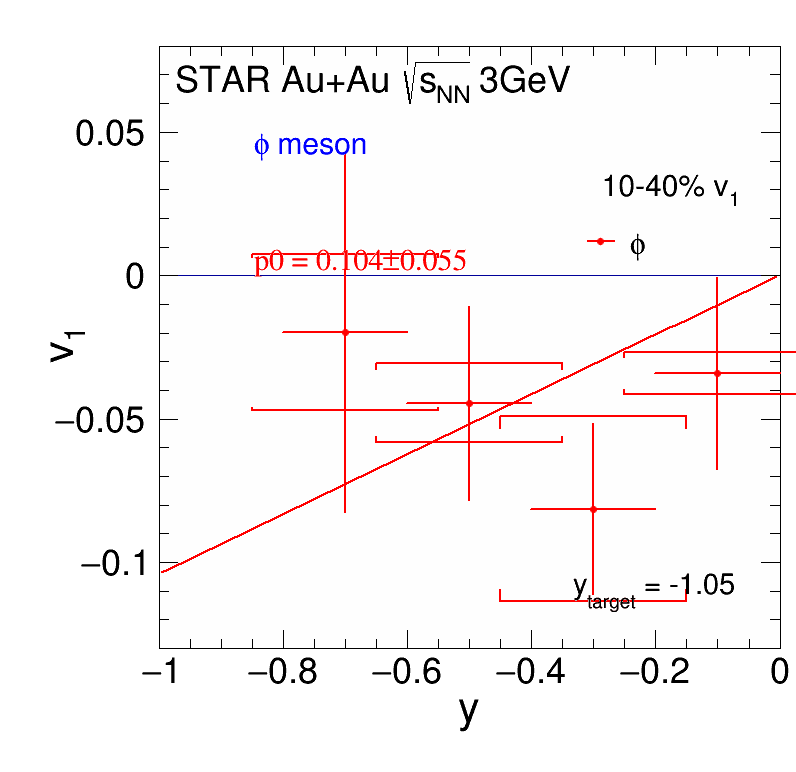
\includegraphics[width=0.49\linewidth]{chapterY/fig/fig1_phi_v1Slop11_10_40.png}
  \caption{$\phi$-meson $v_1$ vs. y, fitted with a linear function cross (0,0).}
\label{phi_dv1dy}
\end{figure}

\subsubsection{$v_2$}

Similar as the $v_1$ analysis, the $\phi$-meson was divided into different $\phi$-$\Psi_{1}$ range and fitted to extract the raw counts and raw $v_2$ as shown in Fig.~\ref{phi_v2} and Fig.~\ref{phi_v2_fit_pT}. The corrected $v_2$ also need to correct the second order event plan resolution which is the same as discussed in the previous section for $\pi$, K and p.

\begin{figure}[h]
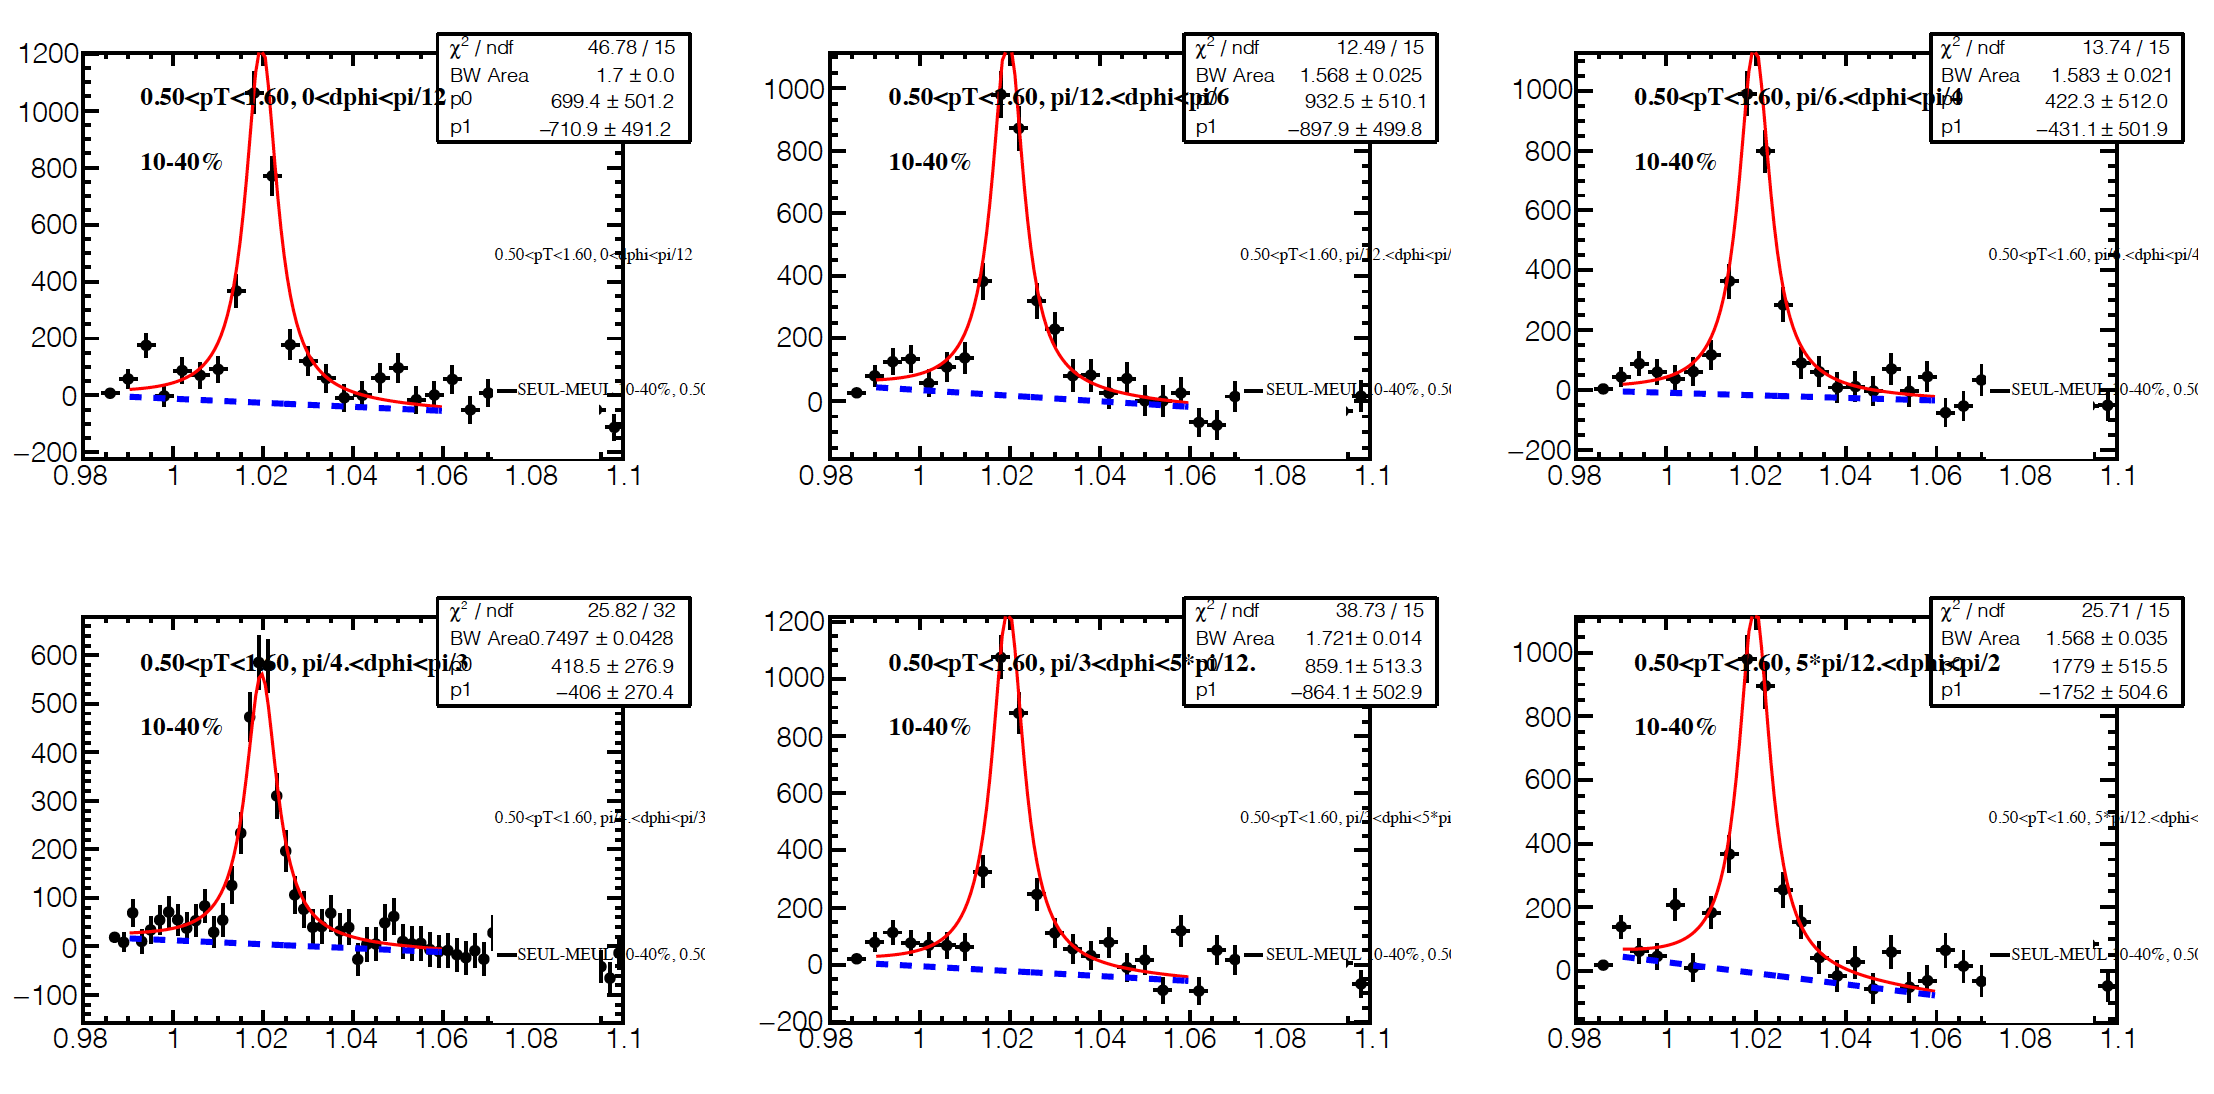
\includegraphics[width=0.98\linewidth]{chapterY/fig/phi_invEP_v2_10_40.png}
\caption{$\phi$-meson signals in several different $\phi$-$\Psi$ range used for the $v_2$ extraction.}
\label{phi_v2}
\end{figure}

\begin{figure}[h]
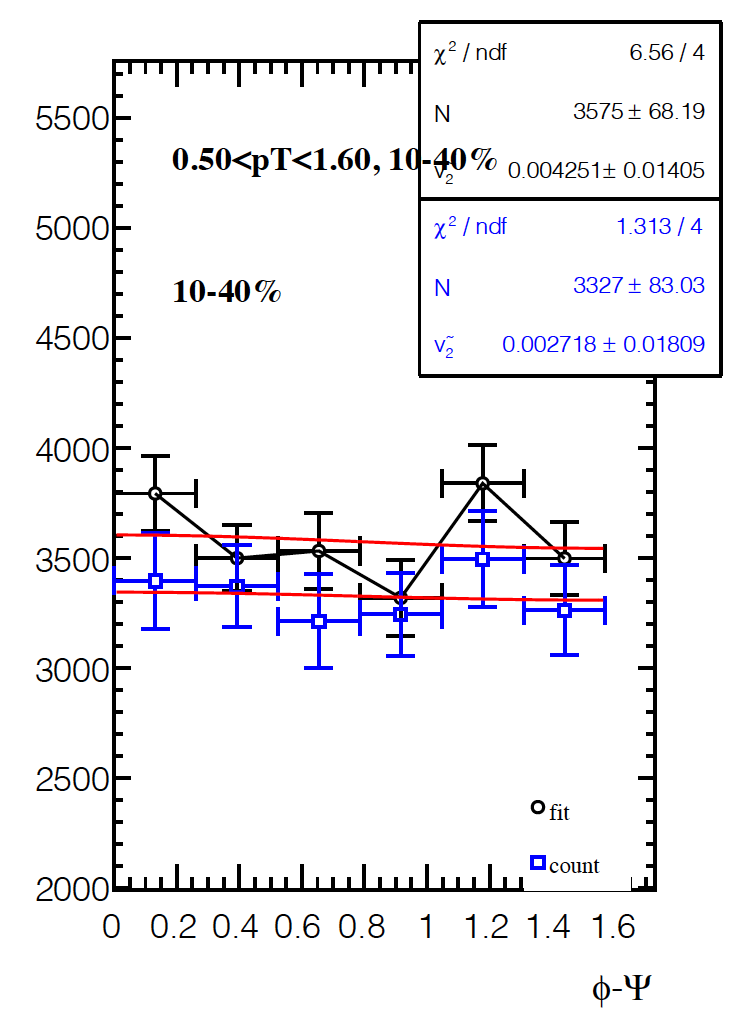
\includegraphics[width=0.45\linewidth]{chapterY/fig/phi_invEP_v2_10_40_fit.png}
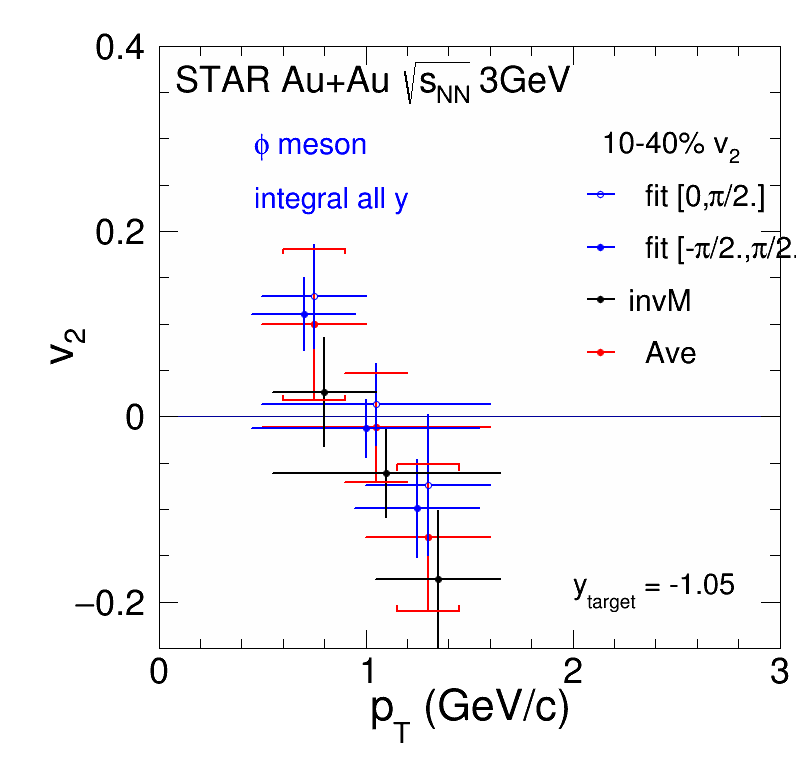
\includegraphics[width=0.49\linewidth]{chapterY/fig/fig1_phi_v2_10_40.png}
  \caption{(left) $\phi$-meson raw counts vs. $\phi-\Psi$ for selected $p_T$ as one example, fitted with the function to extract the raw v2. (right) $\phi$-meson $v_2$ vs. $p_T$, here the three $p_T$ range are from [0.5,1.0],[1.0,1.6],[0.5,1.6].}
\label{phi_v2_fit_pT}
\end{figure}

For the systematic uncertainties, several components were used to evaluate the contribution, basically the same as for the $\phi$-meson spectra analysis: we vary the nHitsFit, dca, n$\sigma_{K}$, 1/$\beta$ for the analysis and we also take different $\phi$-$\Psi_{1}$ fit range for the $v_1$ and $v_2$ extraction and take the difference as the systematic. For each physical variable, since the data precision is not good, we always use the averaged value from all different cuts as the central value to avoid the fluctuations. 

\subsection{Results}
\subsubsection{$v_1$ results for $\phi$-meson}

Fig.~\ref{phi_dv1dy_energy} shows the $\phi$-meson $dv_1/dy$ slop along with the collision energies for the 10-40\% centrality. As see, with the data precision, there is a hint of positive $dv_1/dy$ slop at 3 GeV which is the same trend as $\pi$, K, p, $K_{s}^0$ and $\Lambda$. Fig.~\ref{phi_v2_pT} shows the $\phi$-meson $v_2/n_q$ along with the scaled kinetic momentum $m_T-m_0/n_q$ for the 10-40\% centrality in mid-rapidity. As see, with the data precision, that is really hard to conclude whether the $\phi$-meson follow the NCQ scaling or not.

\begin{figure}[h]
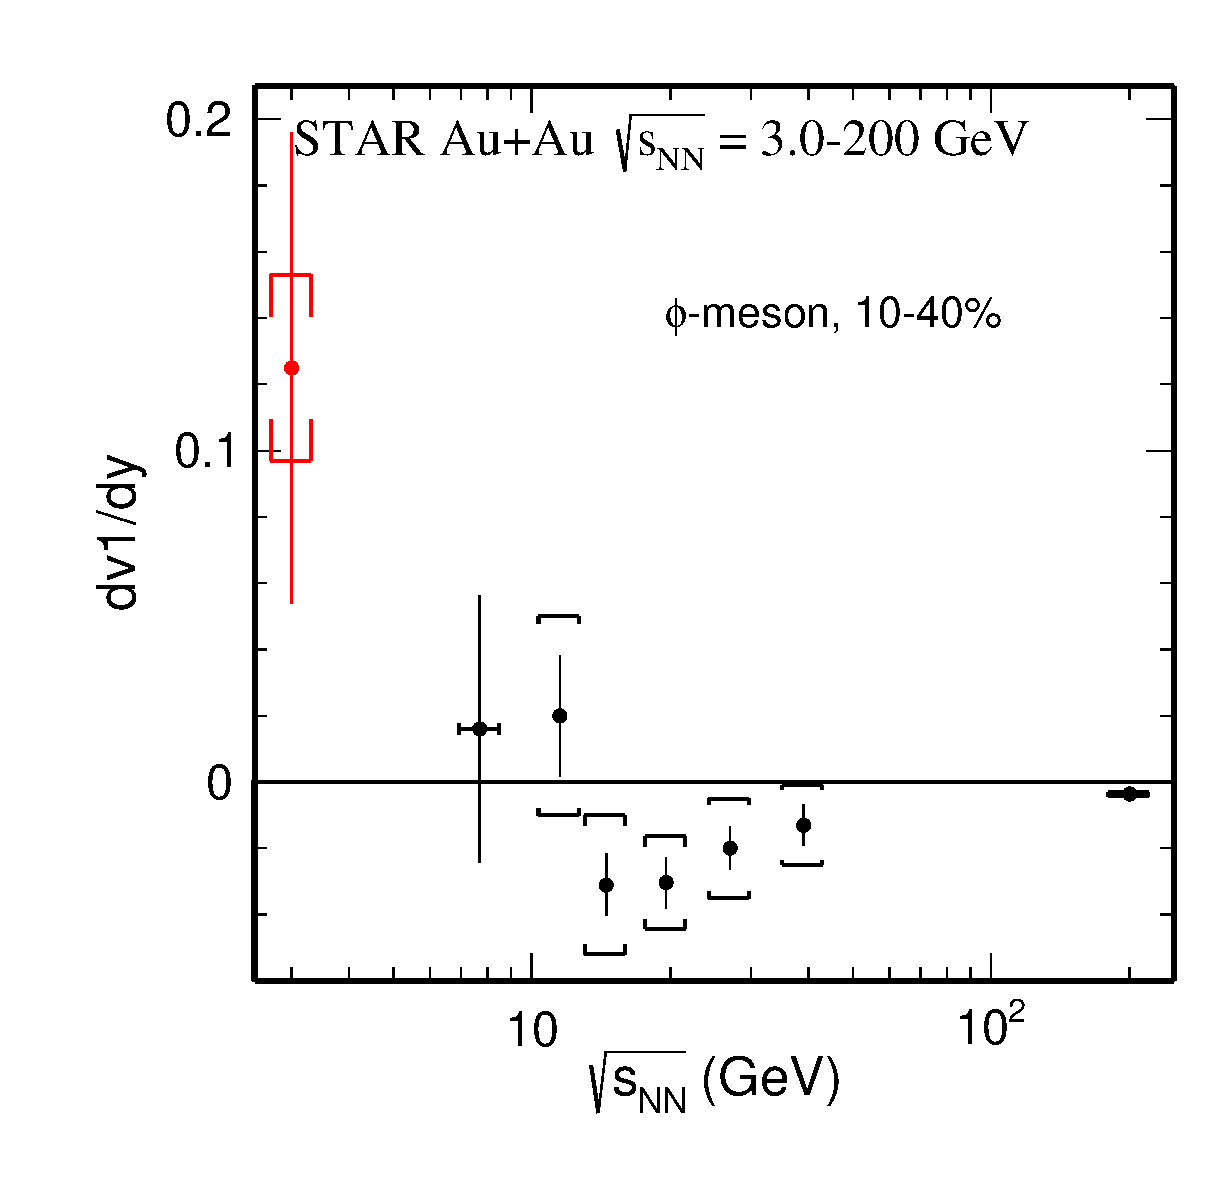
\includegraphics[width=0.6\linewidth]{chapterY/fig/Fffig_dv1_vs_sNN.eps}
\caption{$\phi$-meson d$v_1$/dy slop as a function of collision energies for $10-40\%$ centrality.}
\label{phi_dv1dy_energy}
\end{figure}

\subsubsection{$v_2$ results for $\phi$-meson}

\begin{figure}[h]
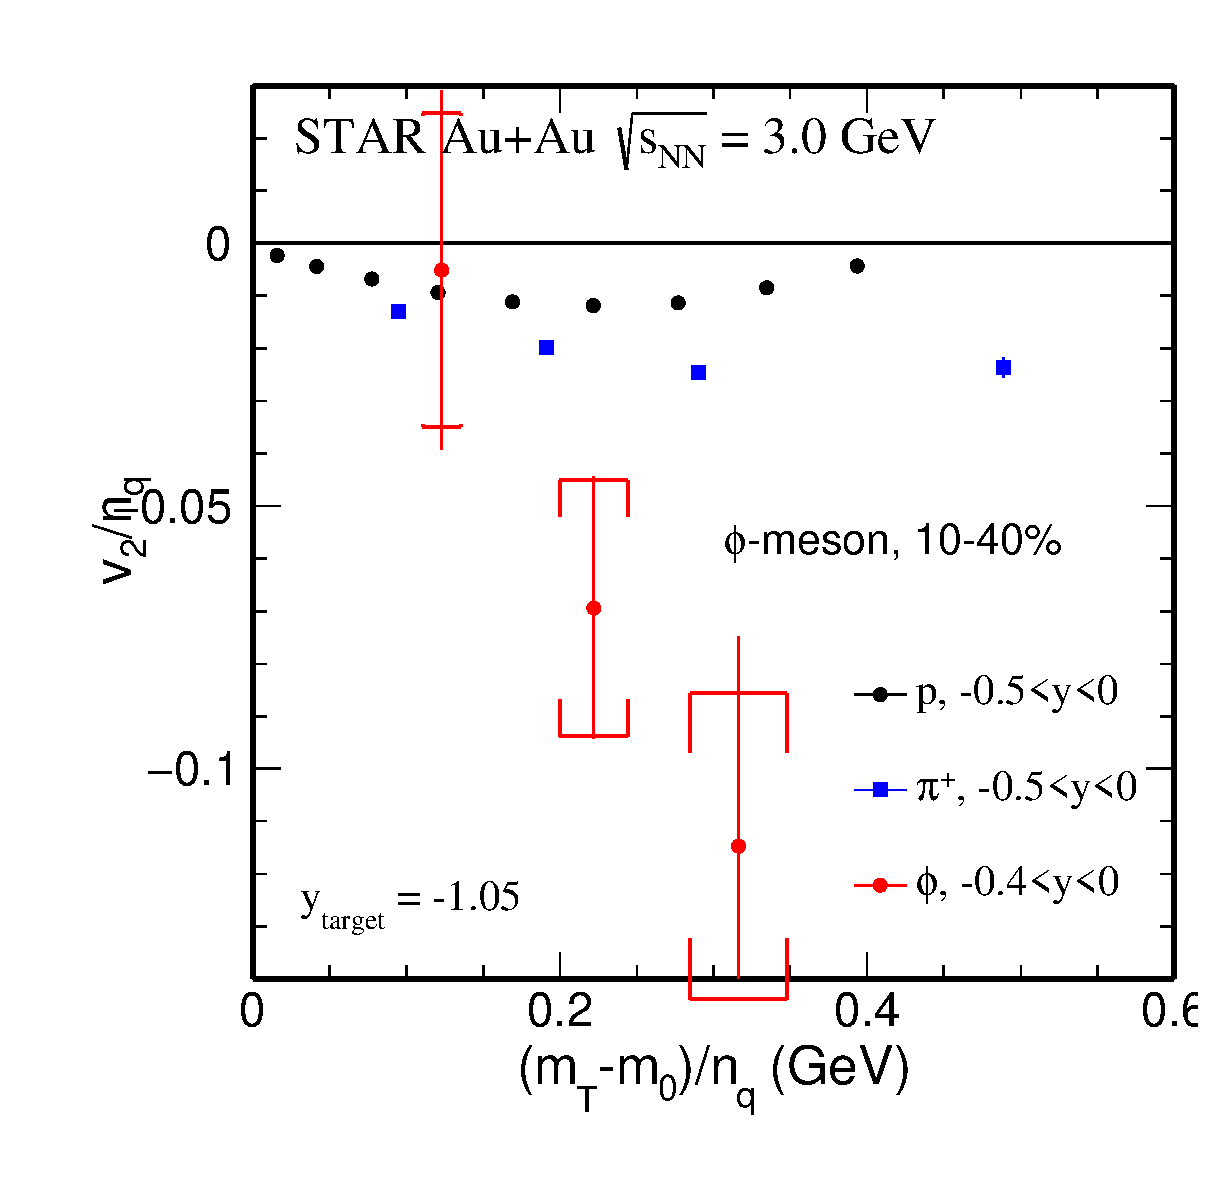
\includegraphics[width=0.6\linewidth]{chapterY/fig/Fffig_v2NCQ_y00p4.eps}
\caption{$\phi$-meson $v_2$/$n_q$ scaling as a function of $m_T-m_0$/$n_q$ for $10-40\%$ centrality and compared with the $\pi$ and p.}
\label{phi_v2_pT}
\end{figure}
